% Part: model-theory
% Chapter: interpolation
% Section: separation

\documentclass[../../../include/open-logic-section]{subfiles}

\begin{document}

\olfileid{mod}{int}{sep}

\olsection{جداسازی \printtoken{P}{sentence}}

پیش از آنکه برهان قضیهٔ درون‌یابی را پیش ببریم، به اندکی زمینه‌سازی
نیاز داریم. درون‌یابِ $!A$ و~$!B$ !!a{sentence}~$!C$ است چنان‌که
$!A \Entails !C$ و $!C \Entails !B$. با عکس نقیض، گزارهٔ دوم هرگاه و
تنها هرگاه $\lnot !B \Entails \lnot !C$. گفته می‌شود
!!^a{sentence}~$!C$ با این خاصیت، $!A$ و~$\lnot !B$ را
\emph{جدا می‌کند}. پس یافتن درون‌یاب برای $!A$ و~$!B$ به یافتن
!!a{sentence}ای فروکاسته می‌شود که $!A$ و~$\lnot !B$ را جدا کند.
مانند بسیاری موارد دیگر، در نظر گرفتن یک تعمیم سودمند خواهد بود:
جمله‌ای که دو \emph{مجموعه} از !!{sentence}s را جدا می‌کند.

\begin{defn}
جملهٔ~$!C$ مجموعه‌های جملهٔ~$\Gamma$ و~$\Delta$ را \emph{جدا می‌کند}
هرگاه و تنها هرگاه $\Gamma \Entails !C$ و
$\Delta \Entails \lnot !C$. اگر چنین !!{sentence}ای وجود نداشته
باشد، $\Gamma$ و~$\Delta$ را \emph{جدایی‌ناپذیر} می‌نامیم.
\end{defn}

روابط شمول میان رده‌های مدل‌های~$\Gamma$، $\Delta$ و~$!C$ در زیر
بازنمایی شده‌اند:
\begin{figure}[h]
  \centering
  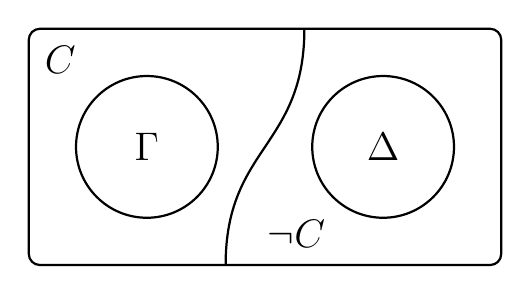
\begin{tikzpicture}[node distance=2cm, auto, thick]
    \draw [rounded corners] (0,0) -- (6,0) -- (6,3) -- (0,3) --  cycle;
    \draw (1.5,1.5) circle (0.9cm);
    \draw (4.5,1.5) circle (0.9cm);
    \path node at (1.5,1.5) {\Large $\Gamma$};
    \path node at (4.5,1.5) {\Large $\Delta$};
    \path node at (0.4,2.6) {\Large $\formula{C}$};
    \path node at (3.4,0.4) {\Large $\lnot \formula{C}$};
    \draw (2.5,0) .. controls (2.5,1.5) and (3.5,1.5) .. (3.5,3);
  \end{tikzpicture}
  \caption{$!C$، $\Gamma$ و~$\Delta$ را جدا می‌کند}
  \ollabel{fig:sep}
\end{figure}


\begin{lem}\ollabel{lem:sep1}
فرض کنید $\Lang{L}_0$ زبانی شامل هر !!{constant}، !!{function} و
!!{predicate} (جز~$\doteq$) باشد که در \emph{هر دو}ی $\Gamma$ و
$\Delta$ رخ می‌دهد، و $\Lang{L}'_0$ با افزودن بی‌نهایت
!!{constant}s تازهٔ $\Obj c_n$ برای $n \ge 0$ به دست آمده باشد. در
این صورت، اگر $\Gamma$ و~$\Delta$ در~$\Lang{L}_0$ جدایی‌ناپذیر باشند،
در~$\Lang{L}'_0$ نیز جدایی‌ناپذیرند.
\end{lem}

\begin{proof}
برهانی غیرمستقیم می‌آوریم: برای رسیدن به تناقض فرض کنید $\Gamma$ و
$\Delta$ در~$\Lang{L}'_0$ جدا شده‌اند. آنگاه برای یک
$!C \in \Lang{L}_0$، $\Gamma \Entails \Subst{!C}{c}{x}$ و
$\Delta \Entails \lnot \Subst{!C}{c}{x}$ (که در آن $c$ یک
!!{constant} تازه است---حالتی که $!C$ بیش از یک چنین !!{constant}ی
دارد مشابه است). بنا بر فشردگی، زیرمجموعه‌های \emph{متناهی}
$\Gamma_0$ از~$\Gamma$ و $\Delta_0$ از~$\Delta$ وجود دارند چنان‌که
$\Gamma_0 \Entails \Subst{!C}{c}{x}$ و
$\Delta_0 \Entails \lnot \Subst{!C}{c}{x}$. بگذارید $!G$ عطف همهٔ
!!{formula}s در~$\Gamma_0$ و $!H$ عطف همهٔ !!{formula}s در~$\Delta_0$
باشد. آنگاه
\begin{align*}
  !G & \Entails \Subst{!C}{c}{x}, & !H  \Entails \lnot \Subst{!C}{c}{x}.
\end{align*}
از گزارهٔ نخست، با تعمیم، داریم $!G \Entails \lforall[x][!C]$؛ و از
گزارهٔ دوم با عکس نقیض، $\Subst{!C}{c}{x} \Entails \lnot !H$، و از
این نیز $\lforall[x][!C] \Entails \lnot !H$. عکس نقیض دوباره نتیجه
می‌دهد $!H \Entails \lnot \lforall[x][!C]$. بنا بر یکنوایی،
\begin{align*}
  \Gamma &\Entails \lforall[x][!C], &
  \Delta & \Entails \lnot \lforall[x][!C],
\end{align*}
پس $\lforall[x][!C]$، $\Gamma$ و~$\Delta$ را در~$\Lang{L}_0$ جدا
می‌کند.
\end{proof}

\begin{lem}\ollabel{lem:sep2}
فرض کنید $\Gamma \cup \{ \lexists[x][!S] \}$ و~$\Delta$
جدایی‌ناپذیرند و $c$ !!{constant} تازه‌ای است که در $\Gamma$،
$\Delta$ یا~$!S$ نیست. آنگاه
$\Gamma \cup \{ \lexists[x][!S], \Subst{!S}{c}{x} \}$ و~$\Delta$
نیز جدایی‌ناپذیرند.
\end{lem}

\begin{proof}
برای رسیدن به تناقض فرض کنید $!C$،
$\Gamma \cup \{\lexists[x][!S], \Subst{!S}{c}{x}\}$ و~$\Delta$ را
جدا می‌کند، درحالی‌که $\Gamma \cup \{\lexists[x][!S] \}$ و~$\Delta$
جدایی‌ناپذیرند. دو حالت را از هم متمایز می‌کنیم:
\begin{enumerate}
\item $c$ در~$!C$ رخ نمی‌دهد: در این حالت
  $\Gamma \cup \{\lexists[x][!S], \lnot!C \}$ ارضاپذیر است (وگرنه
  $!C$، $\Gamma \cup \{\lexists[x][!S] \}$ و~$\Delta$ را جدا
  می‌کند). با افزودن $\Subst{!S}{c}{x}$ نیز ارضاپذیر می‌ماند، پس در
  نهایت $!C$،
  $\Gamma \cup \{ \lexists[x][!S], \Subst{!S}{c}{x} \}$ و~$\Delta$
  را جدا نمی‌کند.
\item $c$ در~$!C$ رخ می‌دهد، به‌گونه‌ای که $!C$ به صورت
  $\Subst{!C}{c}{x}$ است. آنگاه داریم
  \[
  \Gamma \cup \{ \lexists[x][!S], \Subst{!S}{c}{x}\} \Entails \Subst{!C}{c}{x},
  \]
  و ازاین‌رو، بنا بر قضیهٔ استنتاج و تعمیم،
  $\Gamma, \lexists[x][!S] \Entails \lforall[x][(!S \lif !C)]$ و در
  نهایت $\Gamma \cup \{ \lexists[x][!S] \} \Entails
  \lexists[x][!C]$. از سوی دیگر،
  $\Delta \Entails \lnot \Subst{!C}{c}{x}$ و بنابراین با تعمیم
  $\Delta \Entails \lnot \lexists[x][!C]$. پس
  $\Gamma \cup \{\lexists[x][!S] \}$ و~$\Delta$ جدایی‌پذیرند، که
  تناقض است.
\end{enumerate}
\end{proof}

\end{document}
